\section{Spark::Sp\-Stream\-Buffer Class Reference}
\label{classSpark_1_1SpStreamBuffer}\index{Spark::SpStreamBuffer@{Spark::SpStreamBuffer}}
{\tt \#include $<$Sp\-Stream\-Buffer.h$>$}

Collaboration diagram for Spark::Sp\-Stream\-Buffer:\begin{figure}[H]
\begin{center}
\leavevmode
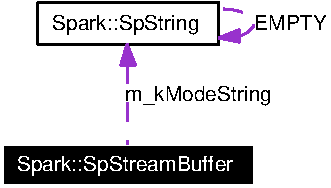
\includegraphics[width=97pt]{classSpark_1_1SpStreamBuffer__coll__graph}
\end{center}
\end{figure}


\subsection{Detailed Description}
A multi-format Open\-GL GPU resident data buffer and render-to-texture (RTT) interface. 

Definition at line 142 of file Sp\-Stream\-Buffer.h.\subsection*{Public Types}
\begin{CompactItemize}
\item 
enum {\bf Update\-Mode} \{ {\bf RT\_\-RENDER\_\-TO\_\-TEXTURE}, 
{\bf RT\_\-COPY\_\-TO\_\-TEXTURE}
 \}
\begin{CompactList}\small\item\em Enumerations:. \item\end{CompactList}\end{CompactItemize}
\subsection*{Public Member Functions}
\begin{CompactItemize}
\item 
{\bf Sp\-Stream\-Buffer} (const char $\ast$str\-Mode=\char`\"{}rgb tex2D\char`\"{})
\begin{CompactList}\small\item\em Construction:. \item\end{CompactList}\item 
{\bf $\sim$Sp\-Stream\-Buffer} ()
\item 
bool {\bf initialize} (int i\-Width, int i\-Height, bool b\-Share\-Objects=true, bool b\-Copy\-Context=false)
\begin{CompactList}\small\item\em Interface:. \item\end{CompactList}\item 
bool {\bf reset} (const char $\ast$ac\-Str\-Mode,...)
\item 
bool {\bf resize} (int i\-Width, int i\-Height)
\item 
unsigned int {\bf copy\-Buffer\-Data} (void $\ast$pv\-Data, int i\-W=-1, int i\-H=-1)
\item 
bool {\bf enable} ()
\item 
bool {\bf enable} ({\bf Sp\-Stream\-Buffer} $\ast$pk\-Current)
\item 
bool {\bf disable} ()
\item 
void {\bf bind} () const
\item 
void {\bf bind\-Depth} () const
\item 
bool {\bf bind\-Buffer} (int i\-Buffer)
\item 
void {\bf enable\-Texture\-Filtering} ()
\item 
void {\bf enable\-Texture\-Target} () const
\begin{CompactList}\small\item\em Enables the texture target appropriate for this render texture. \item\end{CompactList}\item 
void {\bf disable\-Texture\-Target} () const
\begin{CompactList}\small\item\em Disables the texture target appropriate for this render texture. \item\end{CompactList}\item 
unsigned int {\bf get\-Texture\-Id} () const
\begin{CompactList}\small\item\em Returns the texture ID. \item\end{CompactList}\item 
unsigned int {\bf get\-Depth\-Texture\-Id} () const
\begin{CompactList}\small\item\em Returns the depth texture ID. \item\end{CompactList}\item 
unsigned int {\bf get\-Texture\-Target} () const
\begin{CompactList}\small\item\em Returns the texture target this texture is bound to. \item\end{CompactList}\item 
{\bf operator unsigned int} () const
\begin{CompactList}\small\item\em Conversion operator allows {\bf Sp\-Stream\-Buffer}{\rm (p.\,\pageref{classSpark_1_1SpStreamBuffer})} to be passed to GL calls. \item\end{CompactList}\item 
int {\bf get\-Width} () const
\begin{CompactList}\small\item\em Returns the width of the offscreen buffer. \item\end{CompactList}\item 
int {\bf get\-Height} () const
\begin{CompactList}\small\item\em Returns the width of the offscreen buffer. \item\end{CompactList}\item 
int {\bf get\-Max\-S} () const
\begin{CompactList}\small\item\em Returns the maximum S texture coordinate. \item\end{CompactList}\item 
int {\bf get\-Max\-T} () const
\begin{CompactList}\small\item\em Returns the maximum T texture coordinate. \item\end{CompactList}\item 
int {\bf get\-Red\-Bits} () const
\begin{CompactList}\small\item\em Returns the number of red bits allocated. \item\end{CompactList}\item 
int {\bf get\-Green\-Bits} () const
\begin{CompactList}\small\item\em Returns the number of green bits allocated. \item\end{CompactList}\item 
int {\bf get\-Blue\-Bits} () const
\begin{CompactList}\small\item\em Returns the number of blue bits allocated. \item\end{CompactList}\item 
int {\bf get\-Alpha\-Bits} () const
\begin{CompactList}\small\item\em Returns the number of alpha bits allocated. \item\end{CompactList}\item 
int {\bf get\-Depth\-Bits} () const
\begin{CompactList}\small\item\em Returns the number of depth bits allocated. \item\end{CompactList}\item 
int {\bf get\-Stencil\-Bits} () const
\begin{CompactList}\small\item\em Returns the number of stencil bits allocated. \item\end{CompactList}\item 
const {\bf Sp\-String} \& {\bf get\-Mode\-String} () const
\begin{CompactList}\small\item\em Returns the initial mode string used to initialize the buffer. \item\end{CompactList}\item 
bool {\bf is\-Initialized} () const
\begin{CompactList}\small\item\em True if this {\bf Sp\-Stream\-Buffer}{\rm (p.\,\pageref{classSpark_1_1SpStreamBuffer})} has been properly initialized. \item\end{CompactList}\item 
bool {\bf is\-Texture} () const
\begin{CompactList}\small\item\em True if this is a texture and not just an offscreen buffer. \item\end{CompactList}\item 
bool {\bf is\-Depth\-Texture} () const
\begin{CompactList}\small\item\em True if this is a depth texture and not just an offscreen buffer. \item\end{CompactList}\item 
bool {\bf is\-Float\-Texture} () const
\begin{CompactList}\small\item\em True if this is a floating point buffer / texture. \item\end{CompactList}\item 
bool {\bf is\-Double\-Buffered} () const
\begin{CompactList}\small\item\em True if this is a double-buffered pbuffer. \item\end{CompactList}\item 
bool {\bf is\-Rectangle\-Texture} () const
\begin{CompactList}\small\item\em True if this texture has non-power-of-two dimensions. \item\end{CompactList}\item 
bool {\bf has\-Depth} () const
\begin{CompactList}\small\item\em True if this pbuffer has a depth buffer. \item\end{CompactList}\item 
bool {\bf has\-Stencil} () const
\begin{CompactList}\small\item\em True if this pbuffer has a stencil buffer. \item\end{CompactList}\item 
bool {\bf is\-Mip\-Mapped} () const
\begin{CompactList}\small\item\em True if this texture has mipmaps. \item\end{CompactList}\end{CompactItemize}
\subsection*{Static Public Member Functions}
\begin{CompactItemize}
\item 
bool {\bf is\-Power\-Of\-Two} (int n)
\begin{CompactList}\small\item\em Returns true if /param n is an integer power of 2. \item\end{CompactList}\end{CompactItemize}
\subsection*{Protected Types}
\begin{CompactItemize}
\item 
typedef std::pair$<$ {\bf Sp\-String}, {\bf Sp\-String} $>$ {\bf Key\-Val}
\begin{CompactList}\small\item\em Internal Typedefs:. \item\end{CompactList}\item 
typedef std::vector$<$ int $>$ {\bf Int\-Array}
\end{CompactItemize}
\subsection*{Protected Member Functions}
\begin{CompactItemize}
\item 
bool {\bf invalidate} ()
\begin{CompactList}\small\item\em Internal Methods:. \item\end{CompactList}\item 
void {\bf parse\-Mode\-String} (const char $\ast$ac\-Mode\-String, {\bf Int\-Array} \&rk\-Pixel\-Format\-Attribs, {\bf Int\-Array} \&rk\-Pixel\-Buffer\-Attribs)
\item 
{\bf Int\-Array} {\bf parse\-Bit\-Vector} ({\bf Sp\-String} bit\-Vector)
\item 
{\bf Key\-Val} {\bf get\-Key\-Value\-Pair} ({\bf Sp\-String} token)
\item 
bool {\bf verify\-Extensions} ()
\item 
bool {\bf initialize\-Textures} ()
\item 
void {\bf capture\-Buffer} ()
\item 
bool {\bf release\-Bound\-Buffers} ()
\item 
bool {\bf make\-Current} ()
\item 
bool {\bf bind\-Depth\-Buffer} () const
\end{CompactItemize}
\subsection*{Protected Attributes}
\begin{CompactItemize}
\item 
int {\bf m\_\-i\-Width}
\begin{CompactList}\small\item\em Internal Data:. \item\end{CompactList}\item 
int {\bf m\_\-i\-Height}
\item 
bool {\bf m\_\-b\-Is\-Texture}
\item 
bool {\bf m\_\-b\-Is\-Depth\-Texture}
\item 
bool {\bf m\_\-b\-Has\-ARBDepth\-Texture}
\item 
{\bf Update\-Mode} {\bf m\_\-e\-Update\-Mode}
\item 
bool {\bf m\_\-b\-Initialized}
\item 
unsigned int {\bf m\_\-i\-Num\-Aux\-Buffers}
\item 
bool {\bf m\_\-b\-Is\-Buffer\-Bound}
\item 
int {\bf m\_\-i\-Current\-Bound\-Buffer}
\item 
unsigned int {\bf m\_\-ui\-Components}
\item 
unsigned int {\bf m\_\-ui\-Color\-Bits} [4]
\item 
unsigned int {\bf m\_\-ui\-Depth\-Bits}
\item 
unsigned int {\bf m\_\-ui\-Stencil\-Bits}
\item 
bool {\bf m\_\-b\-Is\-Float}
\item 
bool {\bf m\_\-b\-Is\-Double\-Buffered}
\item 
bool {\bf m\_\-b\-Is\-Power\-Of2}
\item 
bool {\bf m\_\-b\-Is\-Rectangle}
\item 
bool {\bf m\_\-b\-Is\-Mip\-Mapped}
\item 
bool {\bf m\_\-b\-Share\-Objects}
\item 
bool {\bf m\_\-b\-Copy\-Context}
\item 
Display $\ast$ {\bf m\_\-pk\-Display}
\item 
GLXContext {\bf m\_\-h\-GLContext}
\item 
GLXPbuffer {\bf m\_\-h\-Pixel\-Buffer}
\item 
GLXDrawable {\bf m\_\-h\-Previous\-Drawable}
\item 
GLXContext {\bf m\_\-h\-Previous\-Context}
\item 
GLenum {\bf m\_\-e\-Texture\-Target}
\item 
unsigned int {\bf m\_\-ui\-Texture\-Id}
\item 
unsigned int {\bf m\_\-ui\-Depth\-Texture\-Id}
\item 
unsigned short $\ast$ {\bf m\_\-aus\-Poor\-Depth\-Texture}
\item 
{\bf Int\-Array} {\bf m\_\-k\-Pixel\-Format\-Attribs}
\item 
{\bf Int\-Array} {\bf m\_\-k\-Pixel\-Buffer\-Attribs}
\item 
{\bf Sp\-String} {\bf m\_\-k\-Mode\-String}
\end{CompactItemize}


\subsection{Member Typedef Documentation}
\index{Spark::SpStreamBuffer@{Spark::Sp\-Stream\-Buffer}!IntArray@{IntArray}}
\index{IntArray@{IntArray}!Spark::SpStreamBuffer@{Spark::Sp\-Stream\-Buffer}}
\subsubsection{\setlength{\rightskip}{0pt plus 5cm}typedef std::vector$<$int$>$ {\bf Spark::Sp\-Stream\-Buffer::Int\-Array}\hspace{0.3cm}{\tt  [protected]}}\label{classSpark_1_1SpStreamBuffer_x1}


Definition at line 319 of file Sp\-Stream\-Buffer.h.\index{Spark::SpStreamBuffer@{Spark::Sp\-Stream\-Buffer}!KeyVal@{KeyVal}}
\index{KeyVal@{KeyVal}!Spark::SpStreamBuffer@{Spark::Sp\-Stream\-Buffer}}
\subsubsection{\setlength{\rightskip}{0pt plus 5cm}typedef std::pair$<${\bf Sp\-String}, {\bf Sp\-String}$>$ {\bf Spark::Sp\-Stream\-Buffer::Key\-Val}\hspace{0.3cm}{\tt  [protected]}}\label{classSpark_1_1SpStreamBuffer_x0}


Internal Typedefs:. 

Definition at line 318 of file Sp\-Stream\-Buffer.h.

Referenced by get\-Key\-Value\-Pair().

\subsection{Member Enumeration Documentation}
\index{Spark::SpStreamBuffer@{Spark::Sp\-Stream\-Buffer}!UpdateMode@{UpdateMode}}
\index{UpdateMode@{UpdateMode}!Spark::SpStreamBuffer@{Spark::Sp\-Stream\-Buffer}}
\subsubsection{\setlength{\rightskip}{0pt plus 5cm}enum {\bf Spark::Sp\-Stream\-Buffer::Update\-Mode}}\label{classSpark_1_1SpStreamBuffer_w2}


Enumerations:. 

\begin{Desc}
\item[Enumeration values: ]\par
\begin{description}
\index{RT_RENDER_TO_TEXTURE@{RT\_\-RENDER\_\-TO\_\-TEXTURE}!Spark::SpStreamBuffer@{Spark::SpStreamBuffer}}\index{Spark::SpStreamBuffer@{Spark::SpStreamBuffer}!RT_RENDER_TO_TEXTURE@{RT\_\-RENDER\_\-TO\_\-TEXTURE}}\item[{\em 
RT\_\-RENDER\_\-TO\_\-TEXTURE\label{classSpark_1_1SpStreamBuffer_w2w0}
}]\index{RT_COPY_TO_TEXTURE@{RT\_\-COPY\_\-TO\_\-TEXTURE}!Spark::SpStreamBuffer@{Spark::SpStreamBuffer}}\index{Spark::SpStreamBuffer@{Spark::SpStreamBuffer}!RT_COPY_TO_TEXTURE@{RT\_\-COPY\_\-TO\_\-TEXTURE}}\item[{\em 
RT\_\-COPY\_\-TO\_\-TEXTURE\label{classSpark_1_1SpStreamBuffer_w2w1}
}]\end{description}
\end{Desc}

Definition at line 148 of file Sp\-Stream\-Buffer.h.

\subsection{Constructor \& Destructor Documentation}
\index{Spark::SpStreamBuffer@{Spark::Sp\-Stream\-Buffer}!SpStreamBuffer@{SpStreamBuffer}}
\index{SpStreamBuffer@{SpStreamBuffer}!Spark::SpStreamBuffer@{Spark::Sp\-Stream\-Buffer}}
\subsubsection{\setlength{\rightskip}{0pt plus 5cm}Sp\-Stream\-Buffer::Sp\-Stream\-Buffer (const char $\ast$ {\em str\-Mode} = {\tt \char`\"{}rgb\ tex2D\char`\"{}})}\label{classSpark_1_1SpStreamBuffer_a0}


Construction:. 

Definition at line 74 of file Sp\-Stream\-Buffer.cpp.

References m\_\-k\-Mode\-String, m\_\-k\-Pixel\-Buffer\-Attribs, m\_\-k\-Pixel\-Format\-Attribs, m\_\-ui\-Color\-Bits, and parse\-Mode\-String().\index{Spark::SpStreamBuffer@{Spark::Sp\-Stream\-Buffer}!~SpStreamBuffer@{$\sim$SpStreamBuffer}}
\index{~SpStreamBuffer@{$\sim$SpStreamBuffer}!Spark::SpStreamBuffer@{Spark::Sp\-Stream\-Buffer}}
\subsubsection{\setlength{\rightskip}{0pt plus 5cm}Sp\-Stream\-Buffer::$\sim${\bf Sp\-Stream\-Buffer} ()}\label{classSpark_1_1SpStreamBuffer_a1}


Definition at line 143 of file Sp\-Stream\-Buffer.cpp.

References invalidate().

\subsection{Member Function Documentation}
\index{Spark::SpStreamBuffer@{Spark::Sp\-Stream\-Buffer}!bind@{bind}}
\index{bind@{bind}!Spark::SpStreamBuffer@{Spark::Sp\-Stream\-Buffer}}
\subsubsection{\setlength{\rightskip}{0pt plus 5cm}void Sp\-Stream\-Buffer::bind () const}\label{classSpark_1_1SpStreamBuffer_a9}


Definition at line 828 of file Sp\-Stream\-Buffer.cpp.

References m\_\-b\-Initialized, m\_\-b\-Is\-Texture, m\_\-e\-Texture\-Target, and m\_\-ui\-Texture\-Id.

Referenced by enable\-Texture\-Filtering().\index{Spark::SpStreamBuffer@{Spark::Sp\-Stream\-Buffer}!bindBuffer@{bindBuffer}}
\index{bindBuffer@{bindBuffer}!Spark::SpStreamBuffer@{Spark::Sp\-Stream\-Buffer}}
\subsubsection{\setlength{\rightskip}{0pt plus 5cm}bool Sp\-Stream\-Buffer::bind\-Buffer (int {\em i\-Buffer})}\label{classSpark_1_1SpStreamBuffer_a11}


Definition at line 848 of file Sp\-Stream\-Buffer.cpp.

References m\_\-b\-Initialized, m\_\-b\-Is\-Buffer\-Bound, m\_\-b\-Is\-Texture, m\_\-e\-Texture\-Target, m\_\-e\-Update\-Mode, m\_\-h\-Pixel\-Buffer, m\_\-i\-Current\-Bound\-Buffer, m\_\-ui\-Texture\-Id, and RT\_\-RENDER\_\-TO\_\-TEXTURE.

Referenced by disable(), enable(), and initialize().\index{Spark::SpStreamBuffer@{Spark::Sp\-Stream\-Buffer}!bindDepth@{bindDepth}}
\index{bindDepth@{bindDepth}!Spark::SpStreamBuffer@{Spark::Sp\-Stream\-Buffer}}
\subsubsection{\setlength{\rightskip}{0pt plus 5cm}void Sp\-Stream\-Buffer::bind\-Depth () const}\label{classSpark_1_1SpStreamBuffer_a10}


Definition at line 838 of file Sp\-Stream\-Buffer.cpp.

References m\_\-b\-Initialized, m\_\-b\-Is\-Depth\-Texture, m\_\-e\-Texture\-Target, and m\_\-ui\-Depth\-Texture\-Id.

Referenced by enable\-Texture\-Filtering().\index{Spark::SpStreamBuffer@{Spark::Sp\-Stream\-Buffer}!bindDepthBuffer@{bindDepthBuffer}}
\index{bindDepthBuffer@{bindDepthBuffer}!Spark::SpStreamBuffer@{Spark::Sp\-Stream\-Buffer}}
\subsubsection{\setlength{\rightskip}{0pt plus 5cm}bool Sp\-Stream\-Buffer::bind\-Depth\-Buffer () const\hspace{0.3cm}{\tt  [protected]}}\label{classSpark_1_1SpStreamBuffer_b9}


Definition at line 877 of file Sp\-Stream\-Buffer.cpp.

References m\_\-b\-Initialized, m\_\-b\-Is\-Depth\-Texture, m\_\-e\-Texture\-Target, m\_\-e\-Update\-Mode, m\_\-h\-Pixel\-Buffer, m\_\-ui\-Depth\-Texture\-Id, and RT\_\-RENDER\_\-TO\_\-TEXTURE.

Referenced by disable(), enable(), and initialize().\index{Spark::SpStreamBuffer@{Spark::Sp\-Stream\-Buffer}!captureBuffer@{captureBuffer}}
\index{captureBuffer@{captureBuffer}!Spark::SpStreamBuffer@{Spark::Sp\-Stream\-Buffer}}
\subsubsection{\setlength{\rightskip}{0pt plus 5cm}void Sp\-Stream\-Buffer::capture\-Buffer ()\hspace{0.3cm}{\tt  [protected]}}\label{classSpark_1_1SpStreamBuffer_b6}


Definition at line 1746 of file Sp\-Stream\-Buffer.cpp.

References m\_\-aus\-Poor\-Depth\-Texture, m\_\-b\-Has\-ARBDepth\-Texture, m\_\-b\-Is\-Depth\-Texture, m\_\-b\-Is\-Texture, m\_\-e\-Texture\-Target, m\_\-e\-Update\-Mode, m\_\-i\-Height, m\_\-i\-Width, m\_\-ui\-Depth\-Texture\-Id, m\_\-ui\-Texture\-Id, and RT\_\-COPY\_\-TO\_\-TEXTURE.

Referenced by disable(), and enable().\index{Spark::SpStreamBuffer@{Spark::Sp\-Stream\-Buffer}!copyBufferData@{copyBufferData}}
\index{copyBufferData@{copyBufferData}!Spark::SpStreamBuffer@{Spark::Sp\-Stream\-Buffer}}
\subsubsection{\setlength{\rightskip}{0pt plus 5cm}unsigned int Spark::Sp\-Stream\-Buffer::copy\-Buffer\-Data (void $\ast$ {\em pv\-Data}, int {\em i\-W} = {\tt -1}, int {\em i\-H} = {\tt -1})\hspace{0.3cm}{\tt  [inline]}}\label{classSpark_1_1SpStreamBuffer_a5}


Definition at line 178 of file Sp\-Stream\-Buffer.h.\index{Spark::SpStreamBuffer@{Spark::Sp\-Stream\-Buffer}!disable@{disable}}
\index{disable@{disable}!Spark::SpStreamBuffer@{Spark::Sp\-Stream\-Buffer}}
\subsubsection{\setlength{\rightskip}{0pt plus 5cm}bool Sp\-Stream\-Buffer::disable ()}\label{classSpark_1_1SpStreamBuffer_a8}


Definition at line 725 of file Sp\-Stream\-Buffer.cpp.

References bind\-Buffer(), bind\-Depth\-Buffer(), capture\-Buffer(), m\_\-b\-Initialized, m\_\-h\-Previous\-Context, m\_\-h\-Previous\-Drawable, m\_\-i\-Current\-Bound\-Buffer, and m\_\-pk\-Display.

Referenced by Spark::Sp\-Vertex\-Noise\-Sb::send\-Output\-To\-Buffer(), and Spark::Sp\-Turbulence\-Op::update\-Output\-Stream().\index{Spark::SpStreamBuffer@{Spark::Sp\-Stream\-Buffer}!disableTextureTarget@{disableTextureTarget}}
\index{disableTextureTarget@{disableTextureTarget}!Spark::SpStreamBuffer@{Spark::Sp\-Stream\-Buffer}}
\subsubsection{\setlength{\rightskip}{0pt plus 5cm}void Spark::Sp\-Stream\-Buffer::disable\-Texture\-Target () const\hspace{0.3cm}{\tt  [inline]}}\label{classSpark_1_1SpStreamBuffer_a14}


Disables the texture target appropriate for this render texture. 

Definition at line 206 of file Sp\-Stream\-Buffer.h.

References m\_\-b\-Initialized, and m\_\-e\-Texture\-Target.\index{Spark::SpStreamBuffer@{Spark::Sp\-Stream\-Buffer}!enable@{enable}}
\index{enable@{enable}!Spark::SpStreamBuffer@{Spark::Sp\-Stream\-Buffer}}
\subsubsection{\setlength{\rightskip}{0pt plus 5cm}bool Sp\-Stream\-Buffer::enable ({\bf Sp\-Stream\-Buffer} $\ast$ {\em pk\-Current})}\label{classSpark_1_1SpStreamBuffer_a7}


Definition at line 760 of file Sp\-Stream\-Buffer.cpp.

References bind\-Buffer(), bind\-Depth\-Buffer(), capture\-Buffer(), enable(), m\_\-b\-Initialized, m\_\-h\-Previous\-Context, m\_\-h\-Previous\-Drawable, m\_\-i\-Current\-Bound\-Buffer, make\-Current(), and release\-Bound\-Buffers().\index{Spark::SpStreamBuffer@{Spark::Sp\-Stream\-Buffer}!enable@{enable}}
\index{enable@{enable}!Spark::SpStreamBuffer@{Spark::Sp\-Stream\-Buffer}}
\subsubsection{\setlength{\rightskip}{0pt plus 5cm}bool Sp\-Stream\-Buffer::enable ()}\label{classSpark_1_1SpStreamBuffer_a6}


Definition at line 697 of file Sp\-Stream\-Buffer.cpp.

References m\_\-b\-Initialized, m\_\-h\-Previous\-Context, m\_\-h\-Previous\-Drawable, make\-Current(), and release\-Bound\-Buffers().

Referenced by enable(), Spark::Sp\-Vertex\-Noise\-Sb::send\-Output\-To\-Buffer(), and Spark::Sp\-Turbulence\-Op::update\-Output\-Stream().\index{Spark::SpStreamBuffer@{Spark::Sp\-Stream\-Buffer}!enableTextureFiltering@{enableTextureFiltering}}
\index{enableTextureFiltering@{enableTextureFiltering}!Spark::SpStreamBuffer@{Spark::Sp\-Stream\-Buffer}}
\subsubsection{\setlength{\rightskip}{0pt plus 5cm}void Sp\-Stream\-Buffer::enable\-Texture\-Filtering ()}\label{classSpark_1_1SpStreamBuffer_a12}


Definition at line 1849 of file Sp\-Stream\-Buffer.cpp.

References bind(), bind\-Depth(), get\-Texture\-Target(), is\-Depth\-Texture(), is\-Float\-Texture(), is\-Mip\-Mapped(), is\-Rectangle\-Texture(), and is\-Texture().\index{Spark::SpStreamBuffer@{Spark::Sp\-Stream\-Buffer}!enableTextureTarget@{enableTextureTarget}}
\index{enableTextureTarget@{enableTextureTarget}!Spark::SpStreamBuffer@{Spark::Sp\-Stream\-Buffer}}
\subsubsection{\setlength{\rightskip}{0pt plus 5cm}void Spark::Sp\-Stream\-Buffer::enable\-Texture\-Target () const\hspace{0.3cm}{\tt  [inline]}}\label{classSpark_1_1SpStreamBuffer_a13}


Enables the texture target appropriate for this render texture. 

Definition at line 202 of file Sp\-Stream\-Buffer.h.

References m\_\-b\-Initialized, and m\_\-e\-Texture\-Target.\index{Spark::SpStreamBuffer@{Spark::Sp\-Stream\-Buffer}!getAlphaBits@{getAlphaBits}}
\index{getAlphaBits@{getAlphaBits}!Spark::SpStreamBuffer@{Spark::Sp\-Stream\-Buffer}}
\subsubsection{\setlength{\rightskip}{0pt plus 5cm}int Spark::Sp\-Stream\-Buffer::get\-Alpha\-Bits () const\hspace{0.3cm}{\tt  [inline]}}\label{classSpark_1_1SpStreamBuffer_a26}


Returns the number of alpha bits allocated. 

Definition at line 254 of file Sp\-Stream\-Buffer.h.

References m\_\-ui\-Color\-Bits.\index{Spark::SpStreamBuffer@{Spark::Sp\-Stream\-Buffer}!getBlueBits@{getBlueBits}}
\index{getBlueBits@{getBlueBits}!Spark::SpStreamBuffer@{Spark::Sp\-Stream\-Buffer}}
\subsubsection{\setlength{\rightskip}{0pt plus 5cm}int Spark::Sp\-Stream\-Buffer::get\-Blue\-Bits () const\hspace{0.3cm}{\tt  [inline]}}\label{classSpark_1_1SpStreamBuffer_a25}


Returns the number of blue bits allocated. 

Definition at line 250 of file Sp\-Stream\-Buffer.h.

References m\_\-ui\-Color\-Bits.\index{Spark::SpStreamBuffer@{Spark::Sp\-Stream\-Buffer}!getDepthBits@{getDepthBits}}
\index{getDepthBits@{getDepthBits}!Spark::SpStreamBuffer@{Spark::Sp\-Stream\-Buffer}}
\subsubsection{\setlength{\rightskip}{0pt plus 5cm}int Spark::Sp\-Stream\-Buffer::get\-Depth\-Bits () const\hspace{0.3cm}{\tt  [inline]}}\label{classSpark_1_1SpStreamBuffer_a27}


Returns the number of depth bits allocated. 

Definition at line 258 of file Sp\-Stream\-Buffer.h.

References m\_\-ui\-Depth\-Bits.\index{Spark::SpStreamBuffer@{Spark::Sp\-Stream\-Buffer}!getDepthTextureId@{getDepthTextureId}}
\index{getDepthTextureId@{getDepthTextureId}!Spark::SpStreamBuffer@{Spark::Sp\-Stream\-Buffer}}
\subsubsection{\setlength{\rightskip}{0pt plus 5cm}unsigned int Spark::Sp\-Stream\-Buffer::get\-Depth\-Texture\-Id () const\hspace{0.3cm}{\tt  [inline]}}\label{classSpark_1_1SpStreamBuffer_a16}


Returns the depth texture ID. 

Definition at line 214 of file Sp\-Stream\-Buffer.h.

References m\_\-ui\-Depth\-Texture\-Id.\index{Spark::SpStreamBuffer@{Spark::Sp\-Stream\-Buffer}!getGreenBits@{getGreenBits}}
\index{getGreenBits@{getGreenBits}!Spark::SpStreamBuffer@{Spark::Sp\-Stream\-Buffer}}
\subsubsection{\setlength{\rightskip}{0pt plus 5cm}int Spark::Sp\-Stream\-Buffer::get\-Green\-Bits () const\hspace{0.3cm}{\tt  [inline]}}\label{classSpark_1_1SpStreamBuffer_a24}


Returns the number of green bits allocated. 

Definition at line 246 of file Sp\-Stream\-Buffer.h.

References m\_\-ui\-Color\-Bits.\index{Spark::SpStreamBuffer@{Spark::Sp\-Stream\-Buffer}!getHeight@{getHeight}}
\index{getHeight@{getHeight}!Spark::SpStreamBuffer@{Spark::Sp\-Stream\-Buffer}}
\subsubsection{\setlength{\rightskip}{0pt plus 5cm}int Spark::Sp\-Stream\-Buffer::get\-Height () const\hspace{0.3cm}{\tt  [inline]}}\label{classSpark_1_1SpStreamBuffer_a20}


Returns the width of the offscreen buffer. 

Definition at line 230 of file Sp\-Stream\-Buffer.h.

References m\_\-i\-Height.

Referenced by Spark::Sp\-Turbulence\-Op::enable\-Output\-Stream(), and Spark::Sp\-Turbulence\-Op::initialize().\index{Spark::SpStreamBuffer@{Spark::Sp\-Stream\-Buffer}!getKeyValuePair@{getKeyValuePair}}
\index{getKeyValuePair@{getKeyValuePair}!Spark::SpStreamBuffer@{Spark::Sp\-Stream\-Buffer}}
\subsubsection{\setlength{\rightskip}{0pt plus 5cm}{\bf Sp\-Stream\-Buffer::Key\-Val} Sp\-Stream\-Buffer::get\-Key\-Value\-Pair ({\bf Sp\-String} {\em token})\hspace{0.3cm}{\tt  [protected]}}\label{classSpark_1_1SpStreamBuffer_b3}


Definition at line 1458 of file Sp\-Stream\-Buffer.cpp.

References Key\-Val.\index{Spark::SpStreamBuffer@{Spark::Sp\-Stream\-Buffer}!getMaxS@{getMaxS}}
\index{getMaxS@{getMaxS}!Spark::SpStreamBuffer@{Spark::Sp\-Stream\-Buffer}}
\subsubsection{\setlength{\rightskip}{0pt plus 5cm}int Spark::Sp\-Stream\-Buffer::get\-Max\-S () const\hspace{0.3cm}{\tt  [inline]}}\label{classSpark_1_1SpStreamBuffer_a21}


Returns the maximum S texture coordinate. 

Definition at line 234 of file Sp\-Stream\-Buffer.h.

References is\-Rectangle\-Texture(), and m\_\-i\-Width.

Referenced by Spark::Sp\-Turbulence\-Op::update\-Output\-Stream().\index{Spark::SpStreamBuffer@{Spark::Sp\-Stream\-Buffer}!getMaxT@{getMaxT}}
\index{getMaxT@{getMaxT}!Spark::SpStreamBuffer@{Spark::Sp\-Stream\-Buffer}}
\subsubsection{\setlength{\rightskip}{0pt plus 5cm}int Spark::Sp\-Stream\-Buffer::get\-Max\-T () const\hspace{0.3cm}{\tt  [inline]}}\label{classSpark_1_1SpStreamBuffer_a22}


Returns the maximum T texture coordinate. 

Definition at line 238 of file Sp\-Stream\-Buffer.h.

References is\-Rectangle\-Texture(), and m\_\-i\-Height.

Referenced by Spark::Sp\-Turbulence\-Op::update\-Output\-Stream().\index{Spark::SpStreamBuffer@{Spark::Sp\-Stream\-Buffer}!getModeString@{getModeString}}
\index{getModeString@{getModeString}!Spark::SpStreamBuffer@{Spark::Sp\-Stream\-Buffer}}
\subsubsection{\setlength{\rightskip}{0pt plus 5cm}const {\bf Sp\-String}\& Spark::Sp\-Stream\-Buffer::get\-Mode\-String () const\hspace{0.3cm}{\tt  [inline]}}\label{classSpark_1_1SpStreamBuffer_a29}


Returns the initial mode string used to initialize the buffer. 

Definition at line 266 of file Sp\-Stream\-Buffer.h.

References m\_\-k\-Mode\-String.\index{Spark::SpStreamBuffer@{Spark::Sp\-Stream\-Buffer}!getRedBits@{getRedBits}}
\index{getRedBits@{getRedBits}!Spark::SpStreamBuffer@{Spark::Sp\-Stream\-Buffer}}
\subsubsection{\setlength{\rightskip}{0pt plus 5cm}int Spark::Sp\-Stream\-Buffer::get\-Red\-Bits () const\hspace{0.3cm}{\tt  [inline]}}\label{classSpark_1_1SpStreamBuffer_a23}


Returns the number of red bits allocated. 

Definition at line 242 of file Sp\-Stream\-Buffer.h.

References m\_\-ui\-Color\-Bits.\index{Spark::SpStreamBuffer@{Spark::Sp\-Stream\-Buffer}!getStencilBits@{getStencilBits}}
\index{getStencilBits@{getStencilBits}!Spark::SpStreamBuffer@{Spark::Sp\-Stream\-Buffer}}
\subsubsection{\setlength{\rightskip}{0pt plus 5cm}int Spark::Sp\-Stream\-Buffer::get\-Stencil\-Bits () const\hspace{0.3cm}{\tt  [inline]}}\label{classSpark_1_1SpStreamBuffer_a28}


Returns the number of stencil bits allocated. 

Definition at line 262 of file Sp\-Stream\-Buffer.h.

References m\_\-ui\-Stencil\-Bits.\index{Spark::SpStreamBuffer@{Spark::Sp\-Stream\-Buffer}!getTextureId@{getTextureId}}
\index{getTextureId@{getTextureId}!Spark::SpStreamBuffer@{Spark::Sp\-Stream\-Buffer}}
\subsubsection{\setlength{\rightskip}{0pt plus 5cm}unsigned int Spark::Sp\-Stream\-Buffer::get\-Texture\-Id () const\hspace{0.3cm}{\tt  [inline]}}\label{classSpark_1_1SpStreamBuffer_a15}


Returns the texture ID. 

Definition at line 210 of file Sp\-Stream\-Buffer.h.

References m\_\-ui\-Texture\-Id.\index{Spark::SpStreamBuffer@{Spark::Sp\-Stream\-Buffer}!getTextureTarget@{getTextureTarget}}
\index{getTextureTarget@{getTextureTarget}!Spark::SpStreamBuffer@{Spark::Sp\-Stream\-Buffer}}
\subsubsection{\setlength{\rightskip}{0pt plus 5cm}unsigned int Spark::Sp\-Stream\-Buffer::get\-Texture\-Target () const\hspace{0.3cm}{\tt  [inline]}}\label{classSpark_1_1SpStreamBuffer_a17}


Returns the texture target this texture is bound to. 

Definition at line 218 of file Sp\-Stream\-Buffer.h.

References m\_\-e\-Texture\-Target.

Referenced by Spark::Sp\-Turbulence\-Op::enable\-Output\-Stream(), enable\-Texture\-Filtering(), Spark::Sp\-Turbulence\-Op::initialize(), and Spark::Sp\-Turbulence\-Op::update\-Output\-Stream().\index{Spark::SpStreamBuffer@{Spark::Sp\-Stream\-Buffer}!getWidth@{getWidth}}
\index{getWidth@{getWidth}!Spark::SpStreamBuffer@{Spark::Sp\-Stream\-Buffer}}
\subsubsection{\setlength{\rightskip}{0pt plus 5cm}int Spark::Sp\-Stream\-Buffer::get\-Width () const\hspace{0.3cm}{\tt  [inline]}}\label{classSpark_1_1SpStreamBuffer_a19}


Returns the width of the offscreen buffer. 

Definition at line 226 of file Sp\-Stream\-Buffer.h.

References m\_\-i\-Width.

Referenced by Spark::Sp\-Turbulence\-Op::enable\-Output\-Stream(), and Spark::Sp\-Turbulence\-Op::initialize().\index{Spark::SpStreamBuffer@{Spark::Sp\-Stream\-Buffer}!hasDepth@{hasDepth}}
\index{hasDepth@{hasDepth}!Spark::SpStreamBuffer@{Spark::Sp\-Stream\-Buffer}}
\subsubsection{\setlength{\rightskip}{0pt plus 5cm}bool Spark::Sp\-Stream\-Buffer::has\-Depth () const\hspace{0.3cm}{\tt  [inline]}}\label{classSpark_1_1SpStreamBuffer_a36}


True if this pbuffer has a depth buffer. 

Definition at line 294 of file Sp\-Stream\-Buffer.h.

References m\_\-ui\-Depth\-Bits.\index{Spark::SpStreamBuffer@{Spark::Sp\-Stream\-Buffer}!hasStencil@{hasStencil}}
\index{hasStencil@{hasStencil}!Spark::SpStreamBuffer@{Spark::Sp\-Stream\-Buffer}}
\subsubsection{\setlength{\rightskip}{0pt plus 5cm}bool Spark::Sp\-Stream\-Buffer::has\-Stencil () const\hspace{0.3cm}{\tt  [inline]}}\label{classSpark_1_1SpStreamBuffer_a37}


True if this pbuffer has a stencil buffer. 

Definition at line 298 of file Sp\-Stream\-Buffer.h.

References m\_\-ui\-Stencil\-Bits.\index{Spark::SpStreamBuffer@{Spark::Sp\-Stream\-Buffer}!initialize@{initialize}}
\index{initialize@{initialize}!Spark::SpStreamBuffer@{Spark::Sp\-Stream\-Buffer}}
\subsubsection{\setlength{\rightskip}{0pt plus 5cm}bool Sp\-Stream\-Buffer::initialize (int {\em i\-Width}, int {\em i\-Height}, bool {\em b\-Share\-Objects} = {\tt true}, bool {\em b\-Copy\-Context} = {\tt false})}\label{classSpark_1_1SpStreamBuffer_a2}


Interface:. 

Call this once before use. Set b\-Share to true to share lists, textures, and program objects between the render texture context and the current active GL context. Definition at line 228 of file Sp\-Stream\-Buffer.cpp.

References bind\-Buffer(), bind\-Depth\-Buffer(), initialize\-Textures(), invalidate(), is\-Power\-Of\-Two(), m\_\-b\-Copy\-Context, m\_\-b\-Initialized, m\_\-b\-Is\-Double\-Buffered, m\_\-b\-Is\-Power\-Of2, m\_\-b\-Share\-Objects, m\_\-h\-GLContext, m\_\-h\-Pixel\-Buffer, m\_\-h\-Previous\-Context, m\_\-h\-Previous\-Drawable, m\_\-i\-Height, m\_\-i\-Width, m\_\-k\-Pixel\-Buffer\-Attribs, m\_\-k\-Pixel\-Format\-Attribs, m\_\-pk\-Display, m\_\-ui\-Color\-Bits, m\_\-ui\-Depth\-Bits, m\_\-ui\-Stencil\-Bits, and verify\-Extensions().

Referenced by resize().\index{Spark::SpStreamBuffer@{Spark::Sp\-Stream\-Buffer}!initializeTextures@{initializeTextures}}
\index{initializeTextures@{initializeTextures}!Spark::SpStreamBuffer@{Spark::Sp\-Stream\-Buffer}}
\subsubsection{\setlength{\rightskip}{0pt plus 5cm}bool Sp\-Stream\-Buffer::initialize\-Textures ()\hspace{0.3cm}{\tt  [protected]}}\label{classSpark_1_1SpStreamBuffer_b5}


Definition at line 1584 of file Sp\-Stream\-Buffer.cpp.

References m\_\-aus\-Poor\-Depth\-Texture, m\_\-b\-Has\-ARBDepth\-Texture, m\_\-b\-Is\-Depth\-Texture, m\_\-b\-Is\-Float, m\_\-b\-Is\-Mip\-Mapped, m\_\-b\-Is\-Rectangle, m\_\-b\-Is\-Texture, m\_\-e\-Texture\-Target, m\_\-e\-Update\-Mode, m\_\-i\-Height, m\_\-i\-Width, m\_\-ui\-Color\-Bits, m\_\-ui\-Components, m\_\-ui\-Depth\-Texture\-Id, m\_\-ui\-Texture\-Id, and RT\_\-COPY\_\-TO\_\-TEXTURE.

Referenced by initialize().\index{Spark::SpStreamBuffer@{Spark::Sp\-Stream\-Buffer}!invalidate@{invalidate}}
\index{invalidate@{invalidate}!Spark::SpStreamBuffer@{Spark::Sp\-Stream\-Buffer}}
\subsubsection{\setlength{\rightskip}{0pt plus 5cm}bool Sp\-Stream\-Buffer::invalidate ()\hspace{0.3cm}{\tt  [protected]}}\label{classSpark_1_1SpStreamBuffer_b0}


Internal Methods:. 

Definition at line 513 of file Sp\-Stream\-Buffer.cpp.

References m\_\-aus\-Poor\-Depth\-Texture, m\_\-b\-Copy\-Context, m\_\-b\-Has\-ARBDepth\-Texture, m\_\-b\-Is\-Depth\-Texture, m\_\-b\-Is\-Texture, m\_\-h\-GLContext, m\_\-h\-Pixel\-Buffer, m\_\-pk\-Display, m\_\-ui\-Color\-Bits, m\_\-ui\-Depth\-Bits, m\_\-ui\-Depth\-Texture\-Id, m\_\-ui\-Stencil\-Bits, and m\_\-ui\-Texture\-Id.

Referenced by initialize(), reset(), and $\sim$Sp\-Stream\-Buffer().\index{Spark::SpStreamBuffer@{Spark::Sp\-Stream\-Buffer}!isDepthTexture@{isDepthTexture}}
\index{isDepthTexture@{isDepthTexture}!Spark::SpStreamBuffer@{Spark::Sp\-Stream\-Buffer}}
\subsubsection{\setlength{\rightskip}{0pt plus 5cm}bool Spark::Sp\-Stream\-Buffer::is\-Depth\-Texture () const\hspace{0.3cm}{\tt  [inline]}}\label{classSpark_1_1SpStreamBuffer_a32}


True if this is a depth texture and not just an offscreen buffer. 

Definition at line 278 of file Sp\-Stream\-Buffer.h.

References m\_\-b\-Is\-Depth\-Texture.

Referenced by enable\-Texture\-Filtering().\index{Spark::SpStreamBuffer@{Spark::Sp\-Stream\-Buffer}!isDoubleBuffered@{isDoubleBuffered}}
\index{isDoubleBuffered@{isDoubleBuffered}!Spark::SpStreamBuffer@{Spark::Sp\-Stream\-Buffer}}
\subsubsection{\setlength{\rightskip}{0pt plus 5cm}bool Spark::Sp\-Stream\-Buffer::is\-Double\-Buffered () const\hspace{0.3cm}{\tt  [inline]}}\label{classSpark_1_1SpStreamBuffer_a34}


True if this is a double-buffered pbuffer. 

Definition at line 286 of file Sp\-Stream\-Buffer.h.

References m\_\-b\-Is\-Double\-Buffered.

Referenced by Spark::Sp\-Vertex\-Noise\-Sb::send\-Output\-To\-Buffer(), and Spark::Sp\-Turbulence\-Op::update\-Output\-Stream().\index{Spark::SpStreamBuffer@{Spark::Sp\-Stream\-Buffer}!isFloatTexture@{isFloatTexture}}
\index{isFloatTexture@{isFloatTexture}!Spark::SpStreamBuffer@{Spark::Sp\-Stream\-Buffer}}
\subsubsection{\setlength{\rightskip}{0pt plus 5cm}bool Spark::Sp\-Stream\-Buffer::is\-Float\-Texture () const\hspace{0.3cm}{\tt  [inline]}}\label{classSpark_1_1SpStreamBuffer_a33}


True if this is a floating point buffer / texture. 

Definition at line 282 of file Sp\-Stream\-Buffer.h.

References m\_\-b\-Is\-Float.

Referenced by enable\-Texture\-Filtering().\index{Spark::SpStreamBuffer@{Spark::Sp\-Stream\-Buffer}!isInitialized@{isInitialized}}
\index{isInitialized@{isInitialized}!Spark::SpStreamBuffer@{Spark::Sp\-Stream\-Buffer}}
\subsubsection{\setlength{\rightskip}{0pt plus 5cm}bool Spark::Sp\-Stream\-Buffer::is\-Initialized () const\hspace{0.3cm}{\tt  [inline]}}\label{classSpark_1_1SpStreamBuffer_a30}


True if this {\bf Sp\-Stream\-Buffer}{\rm (p.\,\pageref{classSpark_1_1SpStreamBuffer})} has been properly initialized. 

Definition at line 270 of file Sp\-Stream\-Buffer.h.

References m\_\-b\-Initialized.

Referenced by reset(), Spark::Sp\-Vertex\-Noise\-Sb::send\-Output\-To\-Buffer(), and Spark::Sp\-Turbulence\-Op::update\-Output\-Stream().\index{Spark::SpStreamBuffer@{Spark::Sp\-Stream\-Buffer}!isMipMapped@{isMipMapped}}
\index{isMipMapped@{isMipMapped}!Spark::SpStreamBuffer@{Spark::Sp\-Stream\-Buffer}}
\subsubsection{\setlength{\rightskip}{0pt plus 5cm}bool Spark::Sp\-Stream\-Buffer::is\-Mip\-Mapped () const\hspace{0.3cm}{\tt  [inline]}}\label{classSpark_1_1SpStreamBuffer_a38}


True if this texture has mipmaps. 

Definition at line 302 of file Sp\-Stream\-Buffer.h.

References m\_\-b\-Is\-Mip\-Mapped.

Referenced by enable\-Texture\-Filtering().\index{Spark::SpStreamBuffer@{Spark::Sp\-Stream\-Buffer}!isPowerOfTwo@{isPowerOfTwo}}
\index{isPowerOfTwo@{isPowerOfTwo}!Spark::SpStreamBuffer@{Spark::Sp\-Stream\-Buffer}}
\subsubsection{\setlength{\rightskip}{0pt plus 5cm}Spark::Sp\-Stream\-Buffer::is\-Power\-Of\-Two (int {\em n})\hspace{0.3cm}{\tt  [inline, static]}}\label{classSpark_1_1SpStreamBuffer_e0}


Returns true if /param n is an integer power of 2. 

Taken from Steve Baker's Cute Code Collection. {\tt http://www.sjbaker.org/steve/software/cute\_\-code.html} Definition at line 312 of file Sp\-Stream\-Buffer.h.

Referenced by initialize().\index{Spark::SpStreamBuffer@{Spark::Sp\-Stream\-Buffer}!isRectangleTexture@{isRectangleTexture}}
\index{isRectangleTexture@{isRectangleTexture}!Spark::SpStreamBuffer@{Spark::Sp\-Stream\-Buffer}}
\subsubsection{\setlength{\rightskip}{0pt plus 5cm}bool Spark::Sp\-Stream\-Buffer::is\-Rectangle\-Texture () const\hspace{0.3cm}{\tt  [inline]}}\label{classSpark_1_1SpStreamBuffer_a35}


True if this texture has non-power-of-two dimensions. 

Definition at line 290 of file Sp\-Stream\-Buffer.h.

References m\_\-b\-Is\-Rectangle.

Referenced by enable\-Texture\-Filtering(), get\-Max\-S(), get\-Max\-T(), and Spark::Sp\-Turbulence\-Op::initialize().\index{Spark::SpStreamBuffer@{Spark::Sp\-Stream\-Buffer}!isTexture@{isTexture}}
\index{isTexture@{isTexture}!Spark::SpStreamBuffer@{Spark::Sp\-Stream\-Buffer}}
\subsubsection{\setlength{\rightskip}{0pt plus 5cm}bool Spark::Sp\-Stream\-Buffer::is\-Texture () const\hspace{0.3cm}{\tt  [inline]}}\label{classSpark_1_1SpStreamBuffer_a31}


True if this is a texture and not just an offscreen buffer. 

Definition at line 274 of file Sp\-Stream\-Buffer.h.

References m\_\-b\-Is\-Texture.

Referenced by enable\-Texture\-Filtering().\index{Spark::SpStreamBuffer@{Spark::Sp\-Stream\-Buffer}!makeCurrent@{makeCurrent}}
\index{makeCurrent@{makeCurrent}!Spark::SpStreamBuffer@{Spark::Sp\-Stream\-Buffer}}
\subsubsection{\setlength{\rightskip}{0pt plus 5cm}bool Sp\-Stream\-Buffer::make\-Current ()\hspace{0.3cm}{\tt  [protected]}}\label{classSpark_1_1SpStreamBuffer_b8}


Definition at line 1830 of file Sp\-Stream\-Buffer.cpp.

References m\_\-h\-GLContext, m\_\-h\-Pixel\-Buffer, and m\_\-pk\-Display.

Referenced by enable().\index{Spark::SpStreamBuffer@{Spark::Sp\-Stream\-Buffer}!operator unsigned int@{operator unsigned int}}
\index{operator unsigned int@{operator unsigned int}!Spark::SpStreamBuffer@{Spark::Sp\-Stream\-Buffer}}
\subsubsection{\setlength{\rightskip}{0pt plus 5cm}Spark::Sp\-Stream\-Buffer::operator unsigned int () const\hspace{0.3cm}{\tt  [inline]}}\label{classSpark_1_1SpStreamBuffer_a18}


Conversion operator allows {\bf Sp\-Stream\-Buffer}{\rm (p.\,\pageref{classSpark_1_1SpStreamBuffer})} to be passed to GL calls. 

Definition at line 222 of file Sp\-Stream\-Buffer.h.

References m\_\-ui\-Texture\-Id.\index{Spark::SpStreamBuffer@{Spark::Sp\-Stream\-Buffer}!parseBitVector@{parseBitVector}}
\index{parseBitVector@{parseBitVector}!Spark::SpStreamBuffer@{Spark::Sp\-Stream\-Buffer}}
\subsubsection{\setlength{\rightskip}{0pt plus 5cm}vector$<$ int $>$ Sp\-Stream\-Buffer::parse\-Bit\-Vector ({\bf Sp\-String} {\em bit\-Vector})\hspace{0.3cm}{\tt  [protected]}}\label{classSpark_1_1SpStreamBuffer_b2}


Definition at line 1473 of file Sp\-Stream\-Buffer.cpp.

References Spark::Sp\-String::Size\-Type.\index{Spark::SpStreamBuffer@{Spark::Sp\-Stream\-Buffer}!parseModeString@{parseModeString}}
\index{parseModeString@{parseModeString}!Spark::SpStreamBuffer@{Spark::Sp\-Stream\-Buffer}}
\subsubsection{\setlength{\rightskip}{0pt plus 5cm}void Spark::Sp\-Stream\-Buffer::parse\-Mode\-String (const char $\ast$ {\em ac\-Mode\-String}, {\bf Int\-Array} \& {\em rk\-Pixel\-Format\-Attribs}, {\bf Int\-Array} \& {\em rk\-Pixel\-Buffer\-Attribs})\hspace{0.3cm}{\tt  [protected]}}\label{classSpark_1_1SpStreamBuffer_b1}




Referenced by reset(), and Sp\-Stream\-Buffer().\index{Spark::SpStreamBuffer@{Spark::Sp\-Stream\-Buffer}!releaseBoundBuffers@{releaseBoundBuffers}}
\index{releaseBoundBuffers@{releaseBoundBuffers}!Spark::SpStreamBuffer@{Spark::Sp\-Stream\-Buffer}}
\subsubsection{\setlength{\rightskip}{0pt plus 5cm}bool Sp\-Stream\-Buffer::release\-Bound\-Buffers ()\hspace{0.3cm}{\tt  [protected]}}\label{classSpark_1_1SpStreamBuffer_b7}


Definition at line 1791 of file Sp\-Stream\-Buffer.cpp.

References m\_\-b\-Is\-Buffer\-Bound, m\_\-b\-Is\-Depth\-Texture, m\_\-b\-Is\-Texture, m\_\-e\-Texture\-Target, m\_\-e\-Update\-Mode, m\_\-h\-Pixel\-Buffer, m\_\-i\-Current\-Bound\-Buffer, m\_\-ui\-Depth\-Texture\-Id, and m\_\-ui\-Texture\-Id.

Referenced by enable().\index{Spark::SpStreamBuffer@{Spark::Sp\-Stream\-Buffer}!reset@{reset}}
\index{reset@{reset}!Spark::SpStreamBuffer@{Spark::Sp\-Stream\-Buffer}}
\subsubsection{\setlength{\rightskip}{0pt plus 5cm}bool Sp\-Stream\-Buffer::reset (const char $\ast$ {\em ac\-Str\-Mode},  {\em ...})}\label{classSpark_1_1SpStreamBuffer_a3}


Definition at line 566 of file Sp\-Stream\-Buffer.cpp.

References invalidate(), is\-Initialized(), m\_\-aus\-Poor\-Depth\-Texture, m\_\-b\-Copy\-Context, m\_\-b\-Has\-ARBDepth\-Texture, m\_\-b\-Initialized, m\_\-b\-Is\-Buffer\-Bound, m\_\-b\-Is\-Depth\-Texture, m\_\-b\-Is\-Double\-Buffered, m\_\-b\-Is\-Float, m\_\-b\-Is\-Mip\-Mapped, m\_\-b\-Is\-Power\-Of2, m\_\-b\-Is\-Rectangle, m\_\-b\-Is\-Texture, m\_\-b\-Share\-Objects, m\_\-e\-Texture\-Target, m\_\-e\-Update\-Mode, m\_\-i\-Current\-Bound\-Buffer, m\_\-i\-Height, m\_\-i\-Num\-Aux\-Buffers, m\_\-i\-Width, m\_\-k\-Pixel\-Buffer\-Attribs, m\_\-k\-Pixel\-Format\-Attribs, m\_\-ui\-Color\-Bits, m\_\-ui\-Depth\-Bits, m\_\-ui\-Depth\-Texture\-Id, m\_\-ui\-Stencil\-Bits, m\_\-ui\-Texture\-Id, parse\-Mode\-String(), and RT\_\-RENDER\_\-TO\_\-TEXTURE.\index{Spark::SpStreamBuffer@{Spark::Sp\-Stream\-Buffer}!resize@{resize}}
\index{resize@{resize}!Spark::SpStreamBuffer@{Spark::Sp\-Stream\-Buffer}}
\subsubsection{\setlength{\rightskip}{0pt plus 5cm}bool Sp\-Stream\-Buffer::resize (int {\em i\-Width}, int {\em i\-Height})}\label{classSpark_1_1SpStreamBuffer_a4}


Definition at line 643 of file Sp\-Stream\-Buffer.cpp.

References initialize(), m\_\-b\-Copy\-Context, m\_\-b\-Initialized, m\_\-b\-Is\-Depth\-Texture, m\_\-b\-Is\-Texture, m\_\-b\-Share\-Objects, m\_\-h\-GLContext, m\_\-h\-Pixel\-Buffer, m\_\-i\-Height, m\_\-i\-Width, m\_\-pk\-Display, m\_\-ui\-Depth\-Texture\-Id, and m\_\-ui\-Texture\-Id.\index{Spark::SpStreamBuffer@{Spark::Sp\-Stream\-Buffer}!verifyExtensions@{verifyExtensions}}
\index{verifyExtensions@{verifyExtensions}!Spark::SpStreamBuffer@{Spark::Sp\-Stream\-Buffer}}
\subsubsection{\setlength{\rightskip}{0pt plus 5cm}bool Sp\-Stream\-Buffer::verify\-Extensions ()\hspace{0.3cm}{\tt  [protected]}}\label{classSpark_1_1SpStreamBuffer_b4}


Definition at line 1503 of file Sp\-Stream\-Buffer.cpp.

References m\_\-b\-Has\-ARBDepth\-Texture, m\_\-b\-Is\-Depth\-Texture, m\_\-b\-Is\-Float, m\_\-b\-Is\-Rectangle, m\_\-b\-Is\-Texture, m\_\-e\-Update\-Mode, and Print\-Extension\-Error().

Referenced by initialize().

\subsection{Member Data Documentation}
\index{Spark::SpStreamBuffer@{Spark::Sp\-Stream\-Buffer}!m_ausPoorDepthTexture@{m\_\-ausPoorDepthTexture}}
\index{m_ausPoorDepthTexture@{m\_\-ausPoorDepthTexture}!Spark::SpStreamBuffer@{Spark::Sp\-Stream\-Buffer}}
\subsubsection{\setlength{\rightskip}{0pt plus 5cm}unsigned short$\ast$ {\bf Spark::Sp\-Stream\-Buffer::m\_\-aus\-Poor\-Depth\-Texture}\hspace{0.3cm}{\tt  [protected]}}\label{classSpark_1_1SpStreamBuffer_p29}


Definition at line 397 of file Sp\-Stream\-Buffer.h.

Referenced by capture\-Buffer(), initialize\-Textures(), invalidate(), and reset().\index{Spark::SpStreamBuffer@{Spark::Sp\-Stream\-Buffer}!m_bCopyContext@{m\_\-bCopyContext}}
\index{m_bCopyContext@{m\_\-bCopyContext}!Spark::SpStreamBuffer@{Spark::Sp\-Stream\-Buffer}}
\subsubsection{\setlength{\rightskip}{0pt plus 5cm}bool {\bf Spark::Sp\-Stream\-Buffer::m\_\-b\-Copy\-Context}\hspace{0.3cm}{\tt  [protected]}}\label{classSpark_1_1SpStreamBuffer_p20}


Definition at line 374 of file Sp\-Stream\-Buffer.h.

Referenced by initialize(), invalidate(), reset(), and resize().\index{Spark::SpStreamBuffer@{Spark::Sp\-Stream\-Buffer}!m_bHasARBDepthTexture@{m\_\-bHasARBDepthTexture}}
\index{m_bHasARBDepthTexture@{m\_\-bHasARBDepthTexture}!Spark::SpStreamBuffer@{Spark::Sp\-Stream\-Buffer}}
\subsubsection{\setlength{\rightskip}{0pt plus 5cm}bool {\bf Spark::Sp\-Stream\-Buffer::m\_\-b\-Has\-ARBDepth\-Texture}\hspace{0.3cm}{\tt  [protected]}}\label{classSpark_1_1SpStreamBuffer_p4}


Definition at line 351 of file Sp\-Stream\-Buffer.h.

Referenced by capture\-Buffer(), initialize\-Textures(), invalidate(), reset(), and verify\-Extensions().\index{Spark::SpStreamBuffer@{Spark::Sp\-Stream\-Buffer}!m_bInitialized@{m\_\-bInitialized}}
\index{m_bInitialized@{m\_\-bInitialized}!Spark::SpStreamBuffer@{Spark::Sp\-Stream\-Buffer}}
\subsubsection{\setlength{\rightskip}{0pt plus 5cm}bool {\bf Spark::Sp\-Stream\-Buffer::m\_\-b\-Initialized}\hspace{0.3cm}{\tt  [protected]}}\label{classSpark_1_1SpStreamBuffer_p6}


Definition at line 355 of file Sp\-Stream\-Buffer.h.

Referenced by bind(), bind\-Buffer(), bind\-Depth(), bind\-Depth\-Buffer(), disable(), disable\-Texture\-Target(), enable(), enable\-Texture\-Target(), initialize(), is\-Initialized(), reset(), and resize().\index{Spark::SpStreamBuffer@{Spark::Sp\-Stream\-Buffer}!m_bIsBufferBound@{m\_\-bIsBufferBound}}
\index{m_bIsBufferBound@{m\_\-bIsBufferBound}!Spark::SpStreamBuffer@{Spark::Sp\-Stream\-Buffer}}
\subsubsection{\setlength{\rightskip}{0pt plus 5cm}bool {\bf Spark::Sp\-Stream\-Buffer::m\_\-b\-Is\-Buffer\-Bound}\hspace{0.3cm}{\tt  [protected]}}\label{classSpark_1_1SpStreamBuffer_p8}


Definition at line 358 of file Sp\-Stream\-Buffer.h.

Referenced by bind\-Buffer(), release\-Bound\-Buffers(), and reset().\index{Spark::SpStreamBuffer@{Spark::Sp\-Stream\-Buffer}!m_bIsDepthTexture@{m\_\-bIsDepthTexture}}
\index{m_bIsDepthTexture@{m\_\-bIsDepthTexture}!Spark::SpStreamBuffer@{Spark::Sp\-Stream\-Buffer}}
\subsubsection{\setlength{\rightskip}{0pt plus 5cm}bool {\bf Spark::Sp\-Stream\-Buffer::m\_\-b\-Is\-Depth\-Texture}\hspace{0.3cm}{\tt  [protected]}}\label{classSpark_1_1SpStreamBuffer_p3}


Definition at line 350 of file Sp\-Stream\-Buffer.h.

Referenced by bind\-Depth(), bind\-Depth\-Buffer(), capture\-Buffer(), initialize\-Textures(), invalidate(), is\-Depth\-Texture(), release\-Bound\-Buffers(), reset(), resize(), and verify\-Extensions().\index{Spark::SpStreamBuffer@{Spark::Sp\-Stream\-Buffer}!m_bIsDoubleBuffered@{m\_\-bIsDoubleBuffered}}
\index{m_bIsDoubleBuffered@{m\_\-bIsDoubleBuffered}!Spark::SpStreamBuffer@{Spark::Sp\-Stream\-Buffer}}
\subsubsection{\setlength{\rightskip}{0pt plus 5cm}bool {\bf Spark::Sp\-Stream\-Buffer::m\_\-b\-Is\-Double\-Buffered}\hspace{0.3cm}{\tt  [protected]}}\label{classSpark_1_1SpStreamBuffer_p15}


Definition at line 368 of file Sp\-Stream\-Buffer.h.

Referenced by initialize(), is\-Double\-Buffered(), and reset().\index{Spark::SpStreamBuffer@{Spark::Sp\-Stream\-Buffer}!m_bIsFloat@{m\_\-bIsFloat}}
\index{m_bIsFloat@{m\_\-bIsFloat}!Spark::SpStreamBuffer@{Spark::Sp\-Stream\-Buffer}}
\subsubsection{\setlength{\rightskip}{0pt plus 5cm}bool {\bf Spark::Sp\-Stream\-Buffer::m\_\-b\-Is\-Float}\hspace{0.3cm}{\tt  [protected]}}\label{classSpark_1_1SpStreamBuffer_p14}


Definition at line 367 of file Sp\-Stream\-Buffer.h.

Referenced by initialize\-Textures(), is\-Float\-Texture(), reset(), and verify\-Extensions().\index{Spark::SpStreamBuffer@{Spark::Sp\-Stream\-Buffer}!m_bIsMipMapped@{m\_\-bIsMipMapped}}
\index{m_bIsMipMapped@{m\_\-bIsMipMapped}!Spark::SpStreamBuffer@{Spark::Sp\-Stream\-Buffer}}
\subsubsection{\setlength{\rightskip}{0pt plus 5cm}bool {\bf Spark::Sp\-Stream\-Buffer::m\_\-b\-Is\-Mip\-Mapped}\hspace{0.3cm}{\tt  [protected]}}\label{classSpark_1_1SpStreamBuffer_p18}


Definition at line 371 of file Sp\-Stream\-Buffer.h.

Referenced by initialize\-Textures(), is\-Mip\-Mapped(), and reset().\index{Spark::SpStreamBuffer@{Spark::Sp\-Stream\-Buffer}!m_bIsPowerOf2@{m\_\-bIsPowerOf2}}
\index{m_bIsPowerOf2@{m\_\-bIsPowerOf2}!Spark::SpStreamBuffer@{Spark::Sp\-Stream\-Buffer}}
\subsubsection{\setlength{\rightskip}{0pt plus 5cm}bool {\bf Spark::Sp\-Stream\-Buffer::m\_\-b\-Is\-Power\-Of2}\hspace{0.3cm}{\tt  [protected]}}\label{classSpark_1_1SpStreamBuffer_p16}


Definition at line 369 of file Sp\-Stream\-Buffer.h.

Referenced by initialize(), and reset().\index{Spark::SpStreamBuffer@{Spark::Sp\-Stream\-Buffer}!m_bIsRectangle@{m\_\-bIsRectangle}}
\index{m_bIsRectangle@{m\_\-bIsRectangle}!Spark::SpStreamBuffer@{Spark::Sp\-Stream\-Buffer}}
\subsubsection{\setlength{\rightskip}{0pt plus 5cm}bool {\bf Spark::Sp\-Stream\-Buffer::m\_\-b\-Is\-Rectangle}\hspace{0.3cm}{\tt  [protected]}}\label{classSpark_1_1SpStreamBuffer_p17}


Definition at line 370 of file Sp\-Stream\-Buffer.h.

Referenced by initialize\-Textures(), is\-Rectangle\-Texture(), reset(), and verify\-Extensions().\index{Spark::SpStreamBuffer@{Spark::Sp\-Stream\-Buffer}!m_bIsTexture@{m\_\-bIsTexture}}
\index{m_bIsTexture@{m\_\-bIsTexture}!Spark::SpStreamBuffer@{Spark::Sp\-Stream\-Buffer}}
\subsubsection{\setlength{\rightskip}{0pt plus 5cm}bool {\bf Spark::Sp\-Stream\-Buffer::m\_\-b\-Is\-Texture}\hspace{0.3cm}{\tt  [protected]}}\label{classSpark_1_1SpStreamBuffer_p2}


Definition at line 349 of file Sp\-Stream\-Buffer.h.

Referenced by bind(), bind\-Buffer(), capture\-Buffer(), initialize\-Textures(), invalidate(), is\-Texture(), release\-Bound\-Buffers(), reset(), resize(), and verify\-Extensions().\index{Spark::SpStreamBuffer@{Spark::Sp\-Stream\-Buffer}!m_bShareObjects@{m\_\-bShareObjects}}
\index{m_bShareObjects@{m\_\-bShareObjects}!Spark::SpStreamBuffer@{Spark::Sp\-Stream\-Buffer}}
\subsubsection{\setlength{\rightskip}{0pt plus 5cm}bool {\bf Spark::Sp\-Stream\-Buffer::m\_\-b\-Share\-Objects}\hspace{0.3cm}{\tt  [protected]}}\label{classSpark_1_1SpStreamBuffer_p19}


Definition at line 373 of file Sp\-Stream\-Buffer.h.

Referenced by initialize(), reset(), and resize().\index{Spark::SpStreamBuffer@{Spark::Sp\-Stream\-Buffer}!m_eTextureTarget@{m\_\-eTextureTarget}}
\index{m_eTextureTarget@{m\_\-eTextureTarget}!Spark::SpStreamBuffer@{Spark::Sp\-Stream\-Buffer}}
\subsubsection{\setlength{\rightskip}{0pt plus 5cm}GLenum {\bf Spark::Sp\-Stream\-Buffer::m\_\-e\-Texture\-Target}\hspace{0.3cm}{\tt  [protected]}}\label{classSpark_1_1SpStreamBuffer_p26}


Definition at line 393 of file Sp\-Stream\-Buffer.h.

Referenced by bind(), bind\-Buffer(), bind\-Depth(), bind\-Depth\-Buffer(), capture\-Buffer(), disable\-Texture\-Target(), enable\-Texture\-Target(), get\-Texture\-Target(), initialize\-Textures(), release\-Bound\-Buffers(), and reset().\index{Spark::SpStreamBuffer@{Spark::Sp\-Stream\-Buffer}!m_eUpdateMode@{m\_\-eUpdateMode}}
\index{m_eUpdateMode@{m\_\-eUpdateMode}!Spark::SpStreamBuffer@{Spark::Sp\-Stream\-Buffer}}
\subsubsection{\setlength{\rightskip}{0pt plus 5cm}{\bf Update\-Mode} {\bf Spark::Sp\-Stream\-Buffer::m\_\-e\-Update\-Mode}\hspace{0.3cm}{\tt  [protected]}}\label{classSpark_1_1SpStreamBuffer_p5}


Definition at line 353 of file Sp\-Stream\-Buffer.h.

Referenced by bind\-Buffer(), bind\-Depth\-Buffer(), capture\-Buffer(), initialize\-Textures(), release\-Bound\-Buffers(), reset(), and verify\-Extensions().\index{Spark::SpStreamBuffer@{Spark::Sp\-Stream\-Buffer}!m_hGLContext@{m\_\-hGLContext}}
\index{m_hGLContext@{m\_\-hGLContext}!Spark::SpStreamBuffer@{Spark::Sp\-Stream\-Buffer}}
\subsubsection{\setlength{\rightskip}{0pt plus 5cm}GLXContext {\bf Spark::Sp\-Stream\-Buffer::m\_\-h\-GLContext}\hspace{0.3cm}{\tt  [protected]}}\label{classSpark_1_1SpStreamBuffer_p22}


Definition at line 385 of file Sp\-Stream\-Buffer.h.

Referenced by initialize(), invalidate(), make\-Current(), and resize().\index{Spark::SpStreamBuffer@{Spark::Sp\-Stream\-Buffer}!m_hPixelBuffer@{m\_\-hPixelBuffer}}
\index{m_hPixelBuffer@{m\_\-hPixelBuffer}!Spark::SpStreamBuffer@{Spark::Sp\-Stream\-Buffer}}
\subsubsection{\setlength{\rightskip}{0pt plus 5cm}GLXPbuffer {\bf Spark::Sp\-Stream\-Buffer::m\_\-h\-Pixel\-Buffer}\hspace{0.3cm}{\tt  [protected]}}\label{classSpark_1_1SpStreamBuffer_p23}


Definition at line 386 of file Sp\-Stream\-Buffer.h.

Referenced by bind\-Buffer(), bind\-Depth\-Buffer(), initialize(), invalidate(), make\-Current(), release\-Bound\-Buffers(), and resize().\index{Spark::SpStreamBuffer@{Spark::Sp\-Stream\-Buffer}!m_hPreviousContext@{m\_\-hPreviousContext}}
\index{m_hPreviousContext@{m\_\-hPreviousContext}!Spark::SpStreamBuffer@{Spark::Sp\-Stream\-Buffer}}
\subsubsection{\setlength{\rightskip}{0pt plus 5cm}GLXContext {\bf Spark::Sp\-Stream\-Buffer::m\_\-h\-Previous\-Context}\hspace{0.3cm}{\tt  [protected]}}\label{classSpark_1_1SpStreamBuffer_p25}


Definition at line 389 of file Sp\-Stream\-Buffer.h.

Referenced by disable(), enable(), and initialize().\index{Spark::SpStreamBuffer@{Spark::Sp\-Stream\-Buffer}!m_hPreviousDrawable@{m\_\-hPreviousDrawable}}
\index{m_hPreviousDrawable@{m\_\-hPreviousDrawable}!Spark::SpStreamBuffer@{Spark::Sp\-Stream\-Buffer}}
\subsubsection{\setlength{\rightskip}{0pt plus 5cm}GLXDrawable {\bf Spark::Sp\-Stream\-Buffer::m\_\-h\-Previous\-Drawable}\hspace{0.3cm}{\tt  [protected]}}\label{classSpark_1_1SpStreamBuffer_p24}


Definition at line 388 of file Sp\-Stream\-Buffer.h.

Referenced by disable(), enable(), and initialize().\index{Spark::SpStreamBuffer@{Spark::Sp\-Stream\-Buffer}!m_iCurrentBoundBuffer@{m\_\-iCurrentBoundBuffer}}
\index{m_iCurrentBoundBuffer@{m\_\-iCurrentBoundBuffer}!Spark::SpStreamBuffer@{Spark::Sp\-Stream\-Buffer}}
\subsubsection{\setlength{\rightskip}{0pt plus 5cm}int {\bf Spark::Sp\-Stream\-Buffer::m\_\-i\-Current\-Bound\-Buffer}\hspace{0.3cm}{\tt  [protected]}}\label{classSpark_1_1SpStreamBuffer_p9}


Definition at line 359 of file Sp\-Stream\-Buffer.h.

Referenced by bind\-Buffer(), disable(), enable(), release\-Bound\-Buffers(), and reset().\index{Spark::SpStreamBuffer@{Spark::Sp\-Stream\-Buffer}!m_iHeight@{m\_\-iHeight}}
\index{m_iHeight@{m\_\-iHeight}!Spark::SpStreamBuffer@{Spark::Sp\-Stream\-Buffer}}
\subsubsection{\setlength{\rightskip}{0pt plus 5cm}int {\bf Spark::Sp\-Stream\-Buffer::m\_\-i\-Height}\hspace{0.3cm}{\tt  [protected]}}\label{classSpark_1_1SpStreamBuffer_p1}


Definition at line 347 of file Sp\-Stream\-Buffer.h.

Referenced by capture\-Buffer(), get\-Height(), get\-Max\-T(), initialize(), initialize\-Textures(), reset(), and resize().\index{Spark::SpStreamBuffer@{Spark::Sp\-Stream\-Buffer}!m_iNumAuxBuffers@{m\_\-iNumAuxBuffers}}
\index{m_iNumAuxBuffers@{m\_\-iNumAuxBuffers}!Spark::SpStreamBuffer@{Spark::Sp\-Stream\-Buffer}}
\subsubsection{\setlength{\rightskip}{0pt plus 5cm}unsigned int {\bf Spark::Sp\-Stream\-Buffer::m\_\-i\-Num\-Aux\-Buffers}\hspace{0.3cm}{\tt  [protected]}}\label{classSpark_1_1SpStreamBuffer_p7}


Definition at line 357 of file Sp\-Stream\-Buffer.h.

Referenced by reset().\index{Spark::SpStreamBuffer@{Spark::Sp\-Stream\-Buffer}!m_iWidth@{m\_\-iWidth}}
\index{m_iWidth@{m\_\-iWidth}!Spark::SpStreamBuffer@{Spark::Sp\-Stream\-Buffer}}
\subsubsection{\setlength{\rightskip}{0pt plus 5cm}int {\bf Spark::Sp\-Stream\-Buffer::m\_\-i\-Width}\hspace{0.3cm}{\tt  [protected]}}\label{classSpark_1_1SpStreamBuffer_p0}


Internal Data:. 

Definition at line 346 of file Sp\-Stream\-Buffer.h.

Referenced by capture\-Buffer(), get\-Max\-S(), get\-Width(), initialize(), initialize\-Textures(), reset(), and resize().\index{Spark::SpStreamBuffer@{Spark::Sp\-Stream\-Buffer}!m_kModeString@{m\_\-kModeString}}
\index{m_kModeString@{m\_\-kModeString}!Spark::SpStreamBuffer@{Spark::Sp\-Stream\-Buffer}}
\subsubsection{\setlength{\rightskip}{0pt plus 5cm}{\bf Sp\-String} {\bf Spark::Sp\-Stream\-Buffer::m\_\-k\-Mode\-String}\hspace{0.3cm}{\tt  [protected]}}\label{classSpark_1_1SpStreamBuffer_p32}


Definition at line 402 of file Sp\-Stream\-Buffer.h.

Referenced by get\-Mode\-String(), and Sp\-Stream\-Buffer().\index{Spark::SpStreamBuffer@{Spark::Sp\-Stream\-Buffer}!m_kPixelBufferAttribs@{m\_\-kPixelBufferAttribs}}
\index{m_kPixelBufferAttribs@{m\_\-kPixelBufferAttribs}!Spark::SpStreamBuffer@{Spark::Sp\-Stream\-Buffer}}
\subsubsection{\setlength{\rightskip}{0pt plus 5cm}{\bf Int\-Array} {\bf Spark::Sp\-Stream\-Buffer::m\_\-k\-Pixel\-Buffer\-Attribs}\hspace{0.3cm}{\tt  [protected]}}\label{classSpark_1_1SpStreamBuffer_p31}


Definition at line 400 of file Sp\-Stream\-Buffer.h.

Referenced by initialize(), reset(), and Sp\-Stream\-Buffer().\index{Spark::SpStreamBuffer@{Spark::Sp\-Stream\-Buffer}!m_kPixelFormatAttribs@{m\_\-kPixelFormatAttribs}}
\index{m_kPixelFormatAttribs@{m\_\-kPixelFormatAttribs}!Spark::SpStreamBuffer@{Spark::Sp\-Stream\-Buffer}}
\subsubsection{\setlength{\rightskip}{0pt plus 5cm}{\bf Int\-Array} {\bf Spark::Sp\-Stream\-Buffer::m\_\-k\-Pixel\-Format\-Attribs}\hspace{0.3cm}{\tt  [protected]}}\label{classSpark_1_1SpStreamBuffer_p30}


Definition at line 399 of file Sp\-Stream\-Buffer.h.

Referenced by initialize(), reset(), and Sp\-Stream\-Buffer().\index{Spark::SpStreamBuffer@{Spark::Sp\-Stream\-Buffer}!m_pkDisplay@{m\_\-pkDisplay}}
\index{m_pkDisplay@{m\_\-pkDisplay}!Spark::SpStreamBuffer@{Spark::Sp\-Stream\-Buffer}}
\subsubsection{\setlength{\rightskip}{0pt plus 5cm}Display$\ast$ {\bf Spark::Sp\-Stream\-Buffer::m\_\-pk\-Display}\hspace{0.3cm}{\tt  [protected]}}\label{classSpark_1_1SpStreamBuffer_p21}


Definition at line 384 of file Sp\-Stream\-Buffer.h.

Referenced by disable(), initialize(), invalidate(), make\-Current(), and resize().\index{Spark::SpStreamBuffer@{Spark::Sp\-Stream\-Buffer}!m_uiColorBits@{m\_\-uiColorBits}}
\index{m_uiColorBits@{m\_\-uiColorBits}!Spark::SpStreamBuffer@{Spark::Sp\-Stream\-Buffer}}
\subsubsection{\setlength{\rightskip}{0pt plus 5cm}unsigned int {\bf Spark::Sp\-Stream\-Buffer::m\_\-ui\-Color\-Bits}[4]\hspace{0.3cm}{\tt  [protected]}}\label{classSpark_1_1SpStreamBuffer_p11}


Definition at line 362 of file Sp\-Stream\-Buffer.h.

Referenced by get\-Alpha\-Bits(), get\-Blue\-Bits(), get\-Green\-Bits(), get\-Red\-Bits(), initialize(), initialize\-Textures(), invalidate(), reset(), and Sp\-Stream\-Buffer().\index{Spark::SpStreamBuffer@{Spark::Sp\-Stream\-Buffer}!m_uiComponents@{m\_\-uiComponents}}
\index{m_uiComponents@{m\_\-uiComponents}!Spark::SpStreamBuffer@{Spark::Sp\-Stream\-Buffer}}
\subsubsection{\setlength{\rightskip}{0pt plus 5cm}unsigned int {\bf Spark::Sp\-Stream\-Buffer::m\_\-ui\-Components}\hspace{0.3cm}{\tt  [protected]}}\label{classSpark_1_1SpStreamBuffer_p10}


Definition at line 361 of file Sp\-Stream\-Buffer.h.

Referenced by initialize\-Textures().\index{Spark::SpStreamBuffer@{Spark::Sp\-Stream\-Buffer}!m_uiDepthBits@{m\_\-uiDepthBits}}
\index{m_uiDepthBits@{m\_\-uiDepthBits}!Spark::SpStreamBuffer@{Spark::Sp\-Stream\-Buffer}}
\subsubsection{\setlength{\rightskip}{0pt plus 5cm}unsigned int {\bf Spark::Sp\-Stream\-Buffer::m\_\-ui\-Depth\-Bits}\hspace{0.3cm}{\tt  [protected]}}\label{classSpark_1_1SpStreamBuffer_p12}


Definition at line 363 of file Sp\-Stream\-Buffer.h.

Referenced by get\-Depth\-Bits(), has\-Depth(), initialize(), invalidate(), and reset().\index{Spark::SpStreamBuffer@{Spark::Sp\-Stream\-Buffer}!m_uiDepthTextureId@{m\_\-uiDepthTextureId}}
\index{m_uiDepthTextureId@{m\_\-uiDepthTextureId}!Spark::SpStreamBuffer@{Spark::Sp\-Stream\-Buffer}}
\subsubsection{\setlength{\rightskip}{0pt plus 5cm}unsigned int {\bf Spark::Sp\-Stream\-Buffer::m\_\-ui\-Depth\-Texture\-Id}\hspace{0.3cm}{\tt  [protected]}}\label{classSpark_1_1SpStreamBuffer_p28}


Definition at line 395 of file Sp\-Stream\-Buffer.h.

Referenced by bind\-Depth(), bind\-Depth\-Buffer(), capture\-Buffer(), get\-Depth\-Texture\-Id(), initialize\-Textures(), invalidate(), release\-Bound\-Buffers(), reset(), and resize().\index{Spark::SpStreamBuffer@{Spark::Sp\-Stream\-Buffer}!m_uiStencilBits@{m\_\-uiStencilBits}}
\index{m_uiStencilBits@{m\_\-uiStencilBits}!Spark::SpStreamBuffer@{Spark::Sp\-Stream\-Buffer}}
\subsubsection{\setlength{\rightskip}{0pt plus 5cm}unsigned int {\bf Spark::Sp\-Stream\-Buffer::m\_\-ui\-Stencil\-Bits}\hspace{0.3cm}{\tt  [protected]}}\label{classSpark_1_1SpStreamBuffer_p13}


Definition at line 364 of file Sp\-Stream\-Buffer.h.

Referenced by get\-Stencil\-Bits(), has\-Stencil(), initialize(), invalidate(), and reset().\index{Spark::SpStreamBuffer@{Spark::Sp\-Stream\-Buffer}!m_uiTextureId@{m\_\-uiTextureId}}
\index{m_uiTextureId@{m\_\-uiTextureId}!Spark::SpStreamBuffer@{Spark::Sp\-Stream\-Buffer}}
\subsubsection{\setlength{\rightskip}{0pt plus 5cm}unsigned int {\bf Spark::Sp\-Stream\-Buffer::m\_\-ui\-Texture\-Id}\hspace{0.3cm}{\tt  [protected]}}\label{classSpark_1_1SpStreamBuffer_p27}


Definition at line 394 of file Sp\-Stream\-Buffer.h.

Referenced by bind(), bind\-Buffer(), capture\-Buffer(), get\-Texture\-Id(), initialize\-Textures(), invalidate(), operator unsigned int(), release\-Bound\-Buffers(), reset(), and resize().

The documentation for this class was generated from the following files:\begin{CompactItemize}
\item 
{\bf Sp\-Stream\-Buffer.h}\item 
{\bf Sp\-Stream\-Buffer.cpp}\end{CompactItemize}
